\documentclass[oneside,10pt,a4paper]{report}
\usepackage[a4paper, left=3cm, right=3cm, top=3cm, bottom=3cm, headsep=10mm, footskip=12mm]{geometry}
\usepackage[T1]{fontenc}
\usepackage[ngerman, english]{babel}    % mehrsprachiger Textsatz
% babel: letzte Sprache in Optionen zeigt die Sprache des Dokumentes
% und kann durch den Befehl \selectlanguage{} geaendert werden
% Passen Sie die Optionen des babel-Paketes nach Bedarf an!
\usepackage{float}
\usepackage{graphicx}
\usepackage{url}
\usepackage{pdflscape}
\usepackage{mathtools}
\usepackage{amssymb, amsmath, amstext}
\usepackage{amsthm}
\usepackage{xcolor}
\usepackage{nameref}
\usepackage{siunitx}
\usepackage{makecell}
\usepackage{hyperref}
\usepackage{enumitem}
\usepackage[superscript,biblabel]{cite}
\usepackage{caption}
\usepackage{subcaption}
\usepackage{tabularx} 			% Tabellen erzeugen
\usepackage{multirow}			 % Zeilen in Tabellenbearbeitung
\usepackage{multicol} 			% Spalten in Tabellenbearbeitung 
\usepackage{lmodern}                        % Ersatz fuer Computer Modern-Schriften 
\usepackage{amsmath}                                           % zum besseren Aussehen am Bildschirm
\usepackage{booktabs} % für schönere Tabellen
\usepackage{sidecap}
\usepackage{rotating} % für die Landscape-Umgebung
\usepackage{afterpage}
\definecolor{Bluetitle}{HTML}{1F3864}
\definecolor{softbluetitle}{HTML}{274D7E}
\definecolor{Greyish}{HTML}{5A5A5A}
%\renewcommand{\refname}{Reference}
\usepackage{array,multirow}
\newcommand{\specialcell}[2][c]{%
	\begin{tabular}[#1]{@{}c@{}}#2\end{tabular}}
\usepackage{titlesec}

\titleformat{\chapter}[display]
{\normalfont\bfseries}{}{0pt}{\Huge}

\usepackage{lipsum} 


\begin{document}
	
	\begin{titlepage}
		\begin{center}
			\begin{figure}[h!tbp]
				
\includegraphics[width=\linewidth]{HUlogo.PNG}
			\end{figure}
			\vspace*{2 cm}
			
			\textcolor{Bluetitle}{\textbf{\huge Molekulare Mikrobiologie}}\par
			
			\vspace*{2cm}
			\textcolor{Greyish}{\textbf{Versuchsdurchführende}}\par
			\textcolor{Greyish}{Huyen Anh Nguyen (572309)}\par
			\textcolor{Greyish}{Johanna Laetitia Heide (...)}\par
			
			
			\vspace*{0.5cm}
			\textcolor{Greyish}{\textbf{Versuchsort}}\par
			\textcolor{Greyish}{Haus 14, Kursraum}\par
			\textcolor{Greyish}{Gruppe 3}\par
			
			
			\vspace*{2 cm}
			\textcolor{Greyish}{\textbf{Versuchsleiter}}\par
			\textcolor{Greyish}{Prof. Dr. Marc Erhardt}\par
			\vspace*{0.5cm}
			\textcolor{Greyish}{\textbf{Versuchsbetreuer}}\par
			\textcolor{Greyish}{Dr. Caroline Kühne}\par
			\textcolor{Greyish}{Heidi Landmesser}\par

			
			\vspace*{2 cm}
			\textcolor{Greyish}{Abgabe 31. Januar 2025}\par
			
			
			
		\end{center}
	\end{titlepage}
	
	
	\tableofcontents
	\chapter{Note from the Author}
	Wir erkläres ausdrücklich, dass wir die Anmerkungen zur Anfertigung des Protokolls gelesen und befolgt haben, dass es sich bei der von uns eingereichte Arbeit um eine von uns erstmalig, selbstständig ohne fremde Hilfe verfasste Arbeit handelt und dass wir sämtliche verwendete zulässige Literatur (Fachpublikationen/-bücher), die unverändert oder abgewandelt wiedergeben werden, insbesondere Quellen für Texte, Grafiken, Tabellen und Bilder als solche kenntlich gemacht haben.\\
	Uns ist bewusst, dass Verstöße gegen diese Grundsätze als Täuschung betrachtet und entsprechend der Prüfungsordnung und/oder der Fächerübergreifenden Satzung zur Reglung von Zulassung, Studium und Prüfung der Humboldt-Universität zu Berlin geahndet werden.
	\\
	\\
	Die Versuche werden wie im Skript "Praktikum Molekulare Mikrobiologie" von Dr. Caroline Kühne \cite{Mibi-Script} durchgeführt. Nur bei Abweichungen werden diese in diesen Protokoll aufgeführt. Zudem wird in diesen Protokoll für die einzelnen Versuchen, die verwendete Phagen- und Sallmonella-Stämme aufgelistet, da in den meisten Versuchen, die unterschiedlichen Stämme unter den Studentenen-Gruppen aufgeteilt wurden.
	
	
	
	
	
	\chapter{Insertion mutagenesis using the transposable element T-Pop}	
	
		\section{Einleitung}
		In diesen Experiment wird untersucht, wie viele Gene des Salmonella Chromosom durch die Insertion des T-POP-Transposon in seinem Salmonella-Stamm mit einem fljB-lac Fusion beeinflusst werden.\\
		In den Salmonella Zellen sind die zwei Gene FljB und FliC (Klasse 3 - Proteine) für die Proteine der Filamente verantwortlich\cite{Flagellum}.
		 Der Salmonella-Stanm für diesen Versuch besitzt in seinem fljB-Gen den Mud-lac-Operon, ein Fusionsgen. (MudJ besitzt ein Kanamycin-Resistenz Kassette fusioniert mit den lac-Operon, wobei hier der Kanamycin-Resistenz Kassette durch ein Chloramphenicol-Resistenz Kassette ersetzt wird.)
		Das bedeutet, wenn das fljB-Gen exprimiert wird, wird zugleich auch der lac Operon mit exprimiert, da der lac Operon den fljB Promotor mitbenutzt.
		
		
		\section{Methode}
		
		In Table \ref{tab: exp2-biologisches Material} wurden die in dem Versuch verwendete Biologisches Material aufgeführt.
		
			\begin{table}[H]
			\centering
			\caption{Verwendete biologische Material für die Insertion von Mutagene mittels eines T-Pop Transposon.}
			\label{tab: exp2-biologisches Material}
			\begin{tabular}{ccc}
				\toprule
				Biologisches Material& Stamm & Phänotyp\\
				\midrule
				\multirow{2}{*}{P22 Phagen Lysat} & \multirow{2}{*}{TH3468} & \multirow{2}{*}{\parbox[t]{9cm}{F’128 (pro-lac) zzf-3834::Tn10dTc[del-20 del-25] (T-POP3) / proAB4}}\\
				&&\\
				&&\\
				\multirow{3}{*}{\parbox[t]{3cm}{Recipienten Salmonellazellen}} & \multirow{3}{*}{EM8052} &\multirow{3}{*}{\parbox[t]{9cm}{MvP103 sseC::aphT (Km$^R$) fljB23028::MudJ-Cm (Km in MudJ replaced by FCF)/ pNK2880 (Ap$^R$)}} \\
				&&\\
				&&\\

				\bottomrule			
			\end{tabular}
		\end{table}

		Durchführung siehe Skript \cite{Mibi-Script}.
		
		\section{Ergebnis}
			\begin{table}[H]
			\centering
			\caption{Mittelwert von der Table \ref{tab: exp2-Rohdaten}. Der Transposon T-POP wurde mit dem Phagenstamm TH3468 in die Salmonella-Recipientenstamm EM8052 in den Genom eingefügt. Hier wurde der Mittelwert der Anzahl der Gene ermittelt, die durch die Insertion betroffen sind.}
			\label{tab: exp2-ergebnis}
			\begin{tabular}{ccccccc}
				\toprule
			\multirow{2}{*}{$\#$TcR} & \multirow{2}{*}{Lac$^-$}&\multirow{2}{*}{lac$^-$ (beide Platten)} & \multirow{2}{*}{Tc-dep.-Lac$^-$}& \multirow{2}{*}{Tc-dep.Lac$^+$}& \multirow{2}{*}{Ratio: $\frac{Lac^-}{\#TcR}$}&\multirow{2}{*}{\parbox[*]{1.2cm}{Genes affected}}\\
				&&&&&&\\
				\midrule
				130 & 2 & 1.5 & 0.5 & 0 & 2/130 & 72\\
				\bottomrule			
			\end{tabular}
		\end{table}
		
		Durch die T-POP insertion konnte im Durchschnitt bestimmt werden, dass 72 Gene für die fliB-lac-Expression verantwortlich sind (siehe Table \ref{tab: exp2-ergebnis}).
		\section{Diskussion}
		Für die Expression des fliB-lac-Fusionsproteine sind ca. 60 Gene verantwortlich (Erwartungswert von Dr. Caroline Kühne im Praktukum vorgegeben). Hier wurde ein Wert von 72 affected Genes ermittelt, welches um 20$\%$ höher liegt als der erwartete Wert. Die Daten wurde aus dem Schnitt von 8 verschiedene Gruppe berechnet, wobei die Standardabweichung circa $\pm$ 31 Gene liegt.\\
		Damit die Standardabweichung verringert werden kann, müsste der Versuch nochmal  innerhalb der Gruppen die Replicaplatten mit n=6 für die MacConkey-Tc- und MacConkey-Lac-Tc-Platten wiederholt werden.
		
		

	
	\chapter{The Luria-Delbrück fluctuation test}	
		\section{Einleitung}
		In diesen Versuch werden die Hypothese überprüft, ob Mutation adaptiv oder zufällig passiert.
		Dabei werden zwei Salmonella-Stämme verwendet, ein Wildtyp und eine die eine Mutation in ihren DNA-Reperatursystem besitzt, und mit den Antibiotika Rifampicin behandelt. \\
		Anhand der Anzahl von Kolonienbildenden Einheiten auf den Antibiotika-Platten wird die Mutationsereignis pro Kultur bestimmt und überprüft, ob die Mutation adaptiv oder zufällig passiert ist.
		
		
		\section{Methode}
			\begin{table}[H]
			\centering
			\caption{Verwendete biologische Material für die den Luira-Delbrück Fluktationstest. Die Stämme wurden in E25-Medium (E Salz Minimal Medium mit 0.0025 $\%$ Glukose) kultiviert bevor es im Versuch in E1000 kultiviert wurde.}
			\label{tab: exp4-biologisches Material}
			\begin{tabular}{ccp{7.5cm}}
				\toprule
				Biologisches Material& Stamm & Phänotyp\\
				\midrule
				\multirow{2}{*}{\parbox[t]{2cm}{Salmonella Wildtyp}}  & \multirow{2}{*}{EM7653} & \multirow{2}{*}{MvP103 sseC::aphT (Km$^R$) wildtype}\\
				&&\\
				&&\\
				\multirow{3}{*}{\parbox[t]{2cm}{Salmonella Mutant}} & \multirow{3}{*}{EM8021} &\multirow{3}{*}{MvP103 sseC::aphT (Km$^R$) $\Delta$mutS::FCF (Cm$^R$)} \\
				&&\\
				&&\\
				
				\bottomrule			
			\end{tabular}
		\end{table}
		
		
		\section{Ergebnis}
		\begin{table}[H]
			\centering
			\caption{Inocolum-Tabelle. Koloniezahlen von Wildtyp (EM7653)und Mutant (EM8021) der jeweiligen Gruppen, die auf LB-Rifampicilin- und LB-Platten gewachsen sind.}
			\label{tab: exp4-Ergebnis}
			\begin{tabular}{ccccccc}
				\toprule
				&\multicolumn{3}{c}{WT (EM7653)}&\multicolumn{3}{c}{$\Delta$mutS (EM8021)}\\
				\midrule
				\multirow{3}{*}{\parbox[t]{1cm}{\textbf{Gr-No.}}}&\multirow{3}{*}{\parbox[t]{2cm}{\textbf{$\qquad$N$_t$}}}& \multirow{3}{*}{\parbox[t]{2cm}{\textbf{$\#$ cultures}}}& \multirow{3}{*}{\parbox[t]{2cm}{\textbf{$\#$ cultures with zero mutations}}} &\multirow{3}{*}{\parbox[t]{2cm}{\textbf{$\qquad$N$_t$}}}& \multirow{3}{*}{\parbox[t]{2cm}{\textbf{$\#$ cultures}}}& \multirow{3}{*}{\parbox[t]{2cm}{\textbf{$\#$ cultures with zero mutations}}}\\
				&&&&&&\\
				&&&&&&\\
				\midrule
				1&1.36$\cdot$10$^7$&36&36&1.39$\cdot$10$^7$&36&20\\
				2&6.2$\cdot$10$^4$&36&36&4.6$\cdot$10$^44$&36&36\\
				3&1.085$\cdot$10$^9$&36&36&5.05$\cdot$10$^6$&36&31\\
				4&N/A&36&36&N/A&36&31\\
				5&1.34$\cdot$10$^7$&36&36&1.26$\cdot$10$^7$&36&34\\
				6&2.6$\cdot$10$^9$&36&33&3.95$\cdot$10$^9$&35&0\\
				7&9.2$\cdot$10$^5$&36&36&N/A&36&28\\
				8&N/A&36&36&N/A&36&30\\
				\bottomrule			
			\end{tabular}
		\end{table}
		
		\begin{table}[H]
			\centering
			\caption{Durchschnittliche Poisson Verteilung p$_0$, Mutationsrate a und Mutationsereigis pro Kultur m vom Wildtyp (EM7653) und Mutant (EM8021)}
			\label{tab: exp4-mutationrate}
			\begin{tabular}{ccccccc}
				\toprule
				\multicolumn{3}{c}{WT (EM7653)}&&\multicolumn{3}{c}{$\Delta$mutS (EM8021)}\\
				\midrule
				p$_0$&a&m&&	p$_0$&a&m\\
				\midrule
				0.982& 1.300$\cdot 10^{-9}$&0.017&&0.732 & 2.479$\cdot 10^{-8}$&0.312\\
				\bottomrule			
			\end{tabular}
		\end{table}
		In der Table \ref{tab: exp4-mutationrate} wurden die Poisson Verteilung p$_0$, Mutationsrate a und Mutationsereignis pro Kultur nach folgende Rechnung bestimmt:\\
		(Beispielzahlen wird für die Gruppe 3 eingesetzt)
		
		\begin{equation}\nonumber
			p_0 (WT)= \frac{\# \text{cultures with zero mutations}}{\#\text{cultures}} = \frac{36}{36} = 1
		\end{equation}
		\begin{equation}\nonumber
			m(WT) = -ln(p_0(WT)) = -ln(1) = 0
		\end{equation}
		\begin{equation}\nonumber
			a(WT) = \frac{m(WT)}{N_t(WT)} = \frac{0}{1.085 \cdot 10^9} = 0
		\end{equation}
		
		Diese Rechnung wird für alle Gruppen gemacht und für den Mutantenstamm und dann den Mittelwert genommen.
		
		\section{Diskussion}
	
	\chapter{Phenotypic analysis of type-III protein secretion}
	
		\section{Analysis of protein secretion via the fT3SS in Salmonella mutants using SDS-PAGE and western blot}
	
		\subsection{Einleitung}
		
		\subsection{Methode}
			\begin{table}[H]
				\centering
				\caption{Salmonella-Stämme die für den Versuch der Analyse der Sekretionsprotei mittels SDS-PAGE und Western Blot verwendet wurde.}
				\label{tab: exp6-biologisches Material part1}
				\begin{tabular}{ccp{7.5cm}}
					\toprule
					Biologisches Material& Stamm & Phänotyp\\
					\midrule
					\multirow{2}{*}{\parbox[t]{2cm}{Salmonella Wildtyp}}  & \multirow{2}{*}{EM8016} & \multirow{2}{*}{\parbox[t]{7.5cm}{MvP103 sseC::aphT (Km$^R$) $\Delta$ hin5717::FRT (fliC-ON)}}\\
					&&\\
					&&\\
					\multirow{3}{*}{\parbox[t]{2cm}{Salmonella Mutant}} & \multirow{3}{*}{EM8035} &\multirow{3}{*}{\parbox[t]{7.5cm}{MvP103 sseC::aphT (Km$^R$) $\Delta$hin5717::FRT (fliC-ON) $\Delta$fliP6659::tetRA}} \\
					&&\\
					&&\\
					
					\bottomrule			
				\end{tabular}
			\end{table}
			
			\subsection{Ergebnis}
				\begin{figure}[H]
				\centering
				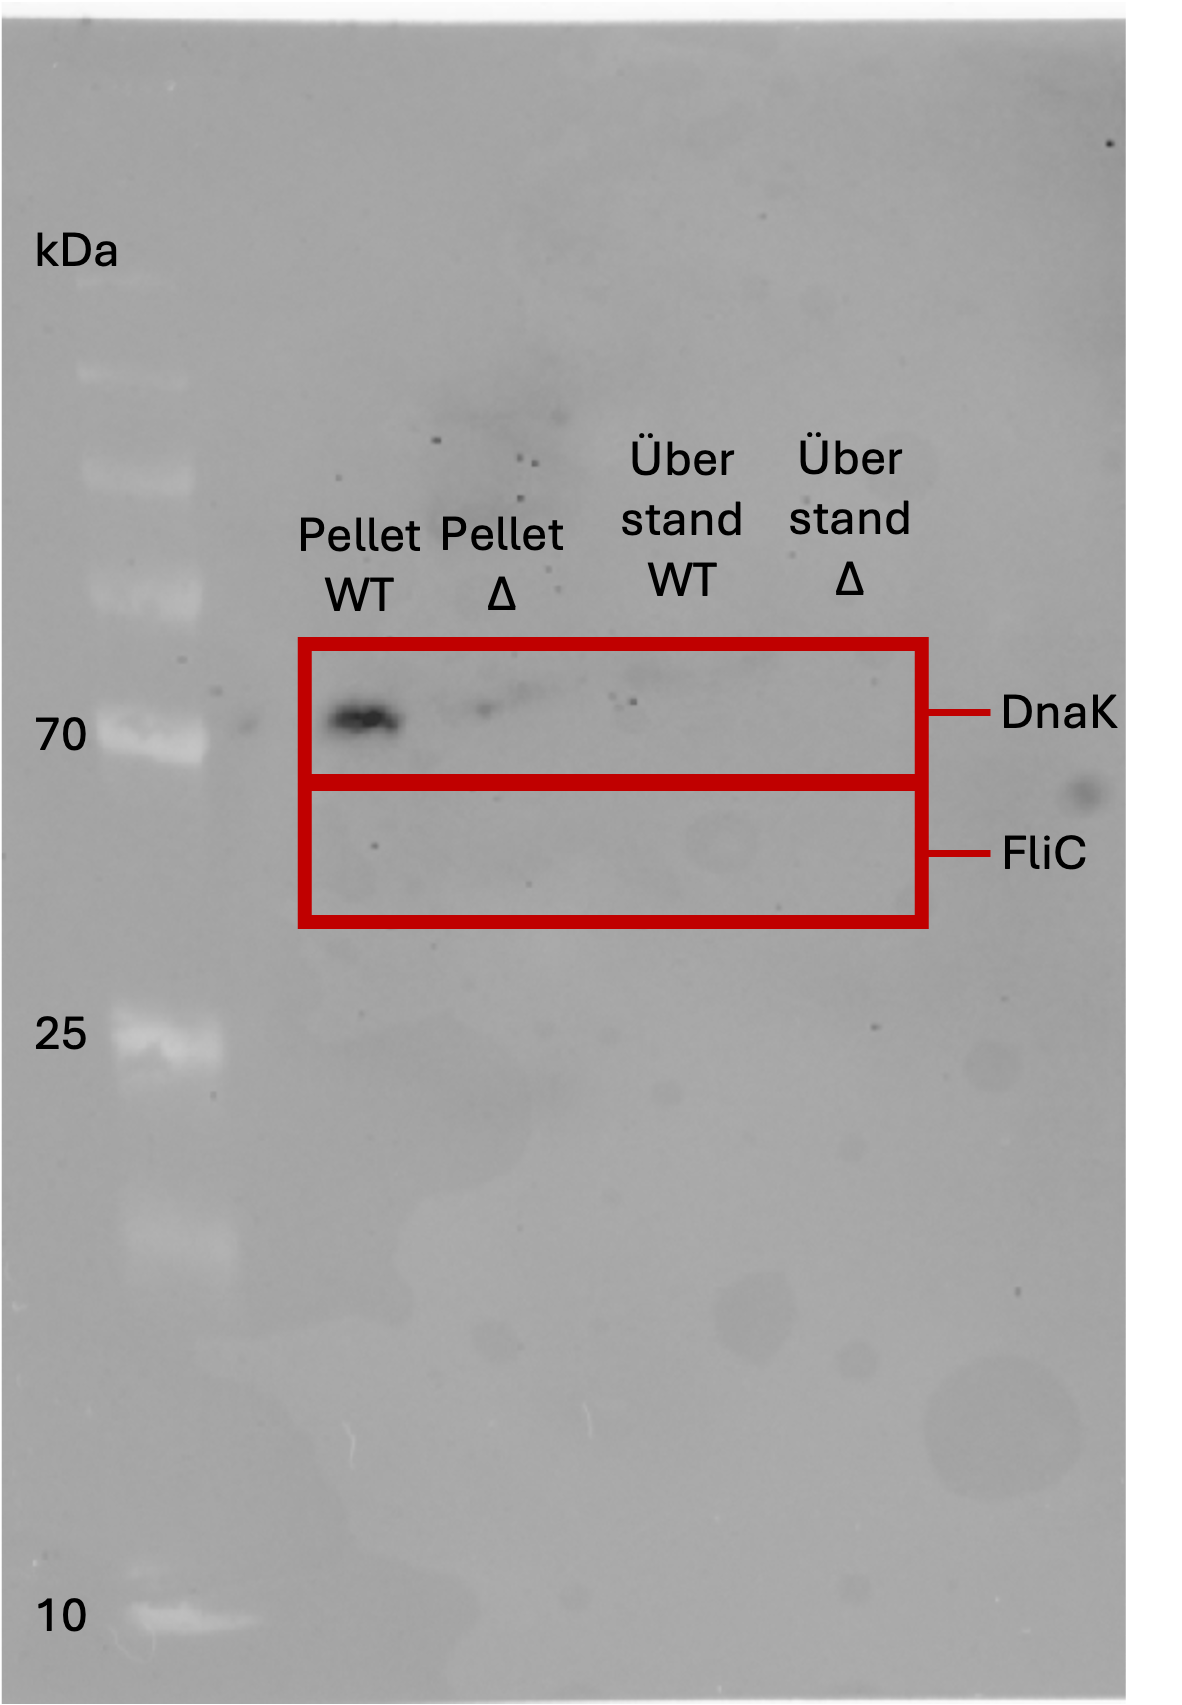
\includegraphics[scale=0.5]{Exp6part1.png}
				\caption{WesternBlot vom Überstand und vom Pellet des Wildtyps EM8016 und Mutant 8035 nach einem SDS-PAGE. Banden wurden mit Antikörper für DnaK und FliC sichtbar gemacht. DnaK gilt hier als Kontrollprotein und hat eine Molekülgröße von 77kDa und FliC eine Größe von 55kDa.}
				\label{fig: Westernblot}
			\end{figure}
			
			
			\subsection{Diskussion}
			
		\section{Luciferase assay to measure gene expression}
		
			\subsection{Einleitung}
			
			\subsection{Methode}
				\begin{table}[H]
				\centering
				\caption{Salmonella-Stämme die für den Luciferase Assay verwendet wurde.}
				\label{tab: exp6-biologisches Material part2}
				\begin{tabular}{ccp{7.5cm}}
					\toprule
					Biologisches Material& Stamm & Phänotyp\\
					\midrule
					\multirow{2}{*}{\parbox[t]{2cm}{Salmonella Wildtyp 1 }}  & \multirow{2}{*}{EM8009} & \multirow{2}{*}{\parbox[t]{7.5cm}{pRG38 (P$_{flhD}$-luxCDABE; Tc$^R$)}}\\
					&&\\
					&&\\
					\multirow{2}{*}{\parbox[t]{2cm}{Salmonella Wildtyp 2}}  & \multirow{2}{*}{EM8008} & \multirow{2}{*}{\parbox[t]{7.5cm}{pRG52 (P$_{flhB}$-luxCDABE; Tc$^R$)}}\\
					&&\\
					&&\\
					\multirow{2}{*}{\parbox[t]{2cm}{Salmonella Wildtyp 3}}  & \multirow{2}{*}{EM8007} & \multirow{2}{*}{\parbox[t]{7.5cm}{pRG19 (P$_{motA}$-luxCDABE; Tc$^R$)}}\\
					&&\\
					&&\\
					\multirow{3}{*}{\parbox[t]{2cm}{Salmonella Mutant 1}} & \multirow{3}{*}{EM8044} &\multirow{3}{*}{\parbox[t]{7.5cm}{$\Delta$flgE22964::FCF / pRG38 (P$_{flhD}$-luxCDABE; Tc$^R$)}} \\
					&&\\
					&&\\
					\multirow{3}{*}{\parbox[t]{2cm}{Salmonella Mutant 2}} & \multirow{3}{*}{EM8045} &\multirow{3}{*}{\parbox[t]{7.5cm}{$\Delta$flgE22964::FCF / pRG52 (P$_{flhB}$-luxCDABE; Tc$^R$)}} \\
					&&\\
					&&\\
					\multirow{3}{*}{\parbox[t]{2cm}{Salmonella Mutant 3}} & \multirow{3}{*}{EM8043} &\multirow{3}{*}{\parbox[t]{7.5cm}{$\Delta$flgE22964::FCF / pRG19 (P$_{flhB}$-luxCDABE; Tc$^R$)}} \\
					&&\\
					&&\\
					
					\bottomrule			
				\end{tabular}
			\end{table}
			
			\section{Ergebnis}
			
				\begin{figure}[H]
				\centering
				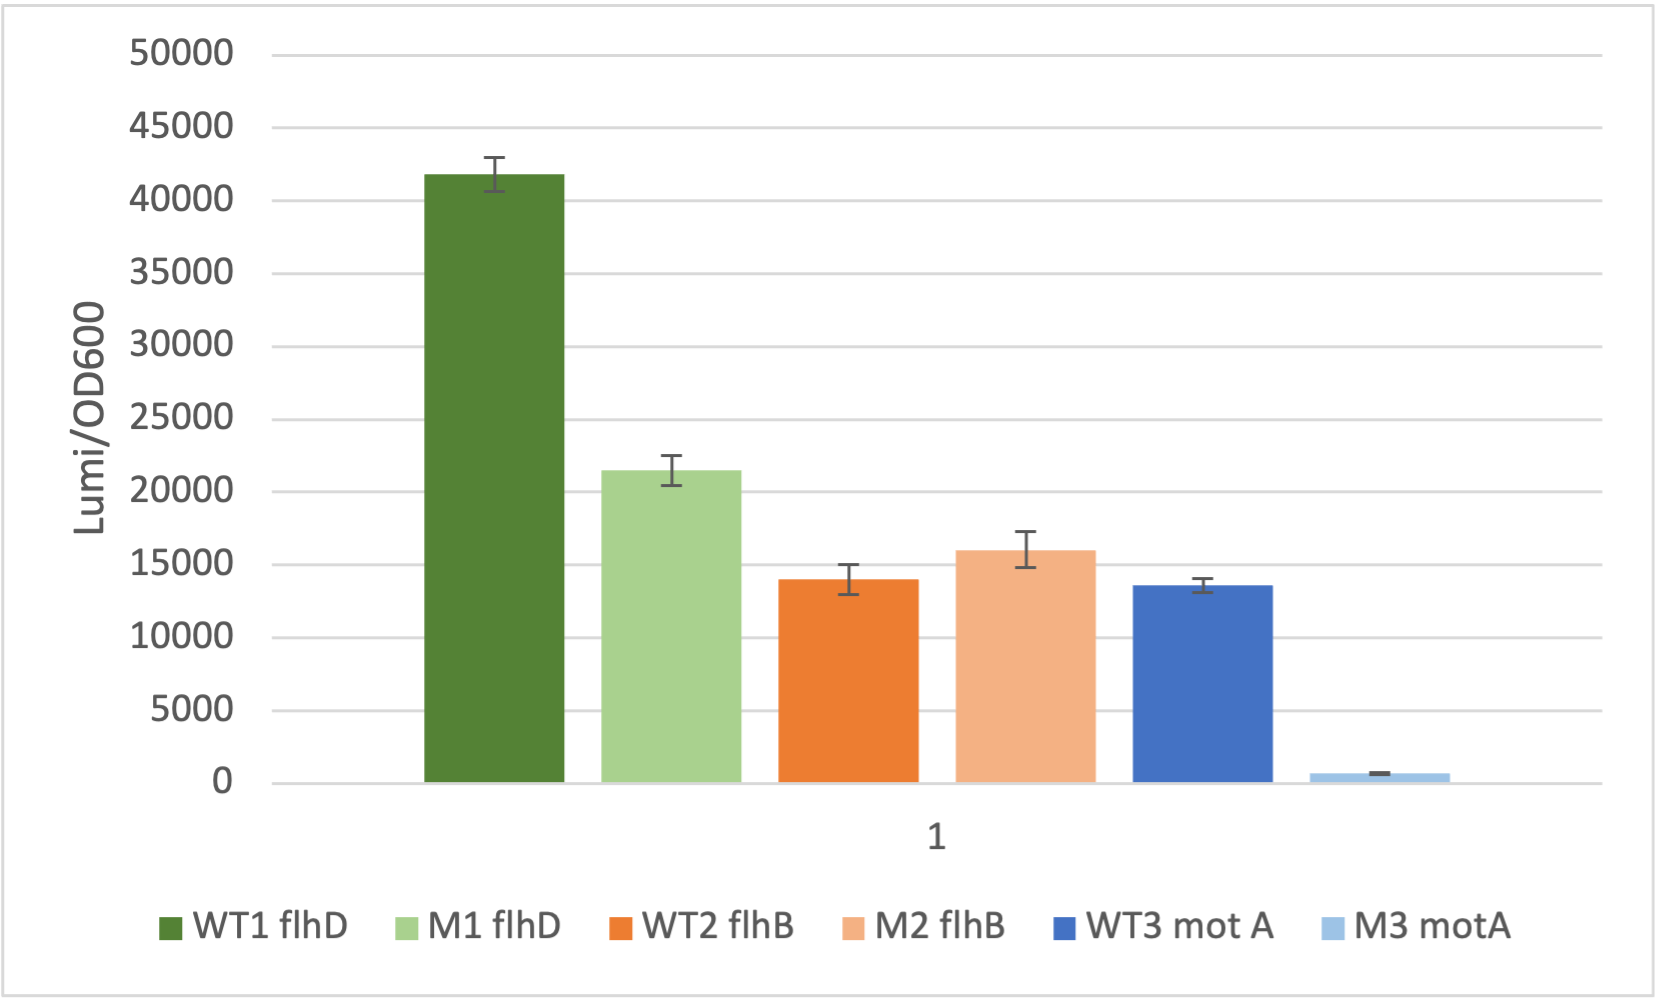
\includegraphics[scale=0.7]{Exp6Lumi.png}
				\caption{Luminiszenz-Verhältnis zu der Zelldichte im Vergleich von Wildtyp und Mutant.}
				\label{fig: Lumi}
			\end{figure}
			
		\section{Motility assay to analyze the swimmng behavor of Salmonella mutants}
		
			\subsection{Einleitung}
			
			\subsection{Methode}
				\begin{table}[H]
				\centering
				\caption{Salmonella-Stämme die für den Motility-Assay verwendet wurde.}
				\label{tab: exp6-biologisches Material part3}
				\begin{tabular}{ccp{5cm}}
					\toprule
					Biologisches Material& Stamm & Phänotyp\\
					\midrule
					\multirow{3}{*}{\parbox[t]{2cm}{Salmonella Wildtyp }}  & \multirow{3}{*}{EM8016} & \multirow{3}{*}{\parbox[t]{4.5cm}{MvP103 sseC::aphT (Km$^R$) $\Delta$hin5717::FRT (fliC-ON)}}\\
					&&\\
					&&\\
					\multirow{3}{*}{\parbox[t]{2cm}{Salmonella Mutant 1}}  & \multirow{3}{*}{EM8033} & \multirow{3}{*}{\parbox[t]{4.5cm}{MvP103 sseC::aphT (Km$^R$) $\Delta$hin5717::FRT (fliC-ON) $\Delta$fliT5758::FCF}}\\
					&&\\
					&&\\
					&&\\
					\multirow{3}{*}{\parbox[t]{2cm}{Salmonella Mutant 2}}  & \multirow{3}{*}{EM8034} & \multirow{3}{*}{\parbox[t]{4.5cm}{MvP103 sseC::aphT (Km$^R$) $\Delta$hin5717::FRT (fliC-ON) $\Delta$fliS5728::FRT}}\\
					&&\\
					&&\\
					&&\\
					\multirow{3}{*}{\parbox[t]{2cm}{Salmonella Mutant 3}} & \multirow{3}{*}{EM8035} &\multirow{3}{*}{\parbox[t]{4.5cm}{MvP103 sseC::aphT (Km$^R$) $\Delta$hin5717::FRT (fliC-ON) $\Delta$fliP6659::tetRA}} \\
					&&\\
					&&\\
					&&\\
					\multirow{3}{*}{\parbox[t]{2cm}{Salmonella Mutant 4}} & \multirow{3}{*}{EM8036} &\multirow{3}{*}{\parbox[t]{4.5cm}{MvP103 sseC::aphT (Km$^R$) $\Delta$hin5717::FRT (fliC-ON) $\Delta$fliC7715::tetRA}} \\
					&&\\
					&&\\
					&&\\
					\bottomrule			
				\end{tabular}
			\end{table}
			
			\subsection{Ergebnis}
			\begin{figure}[H]
				\centering
				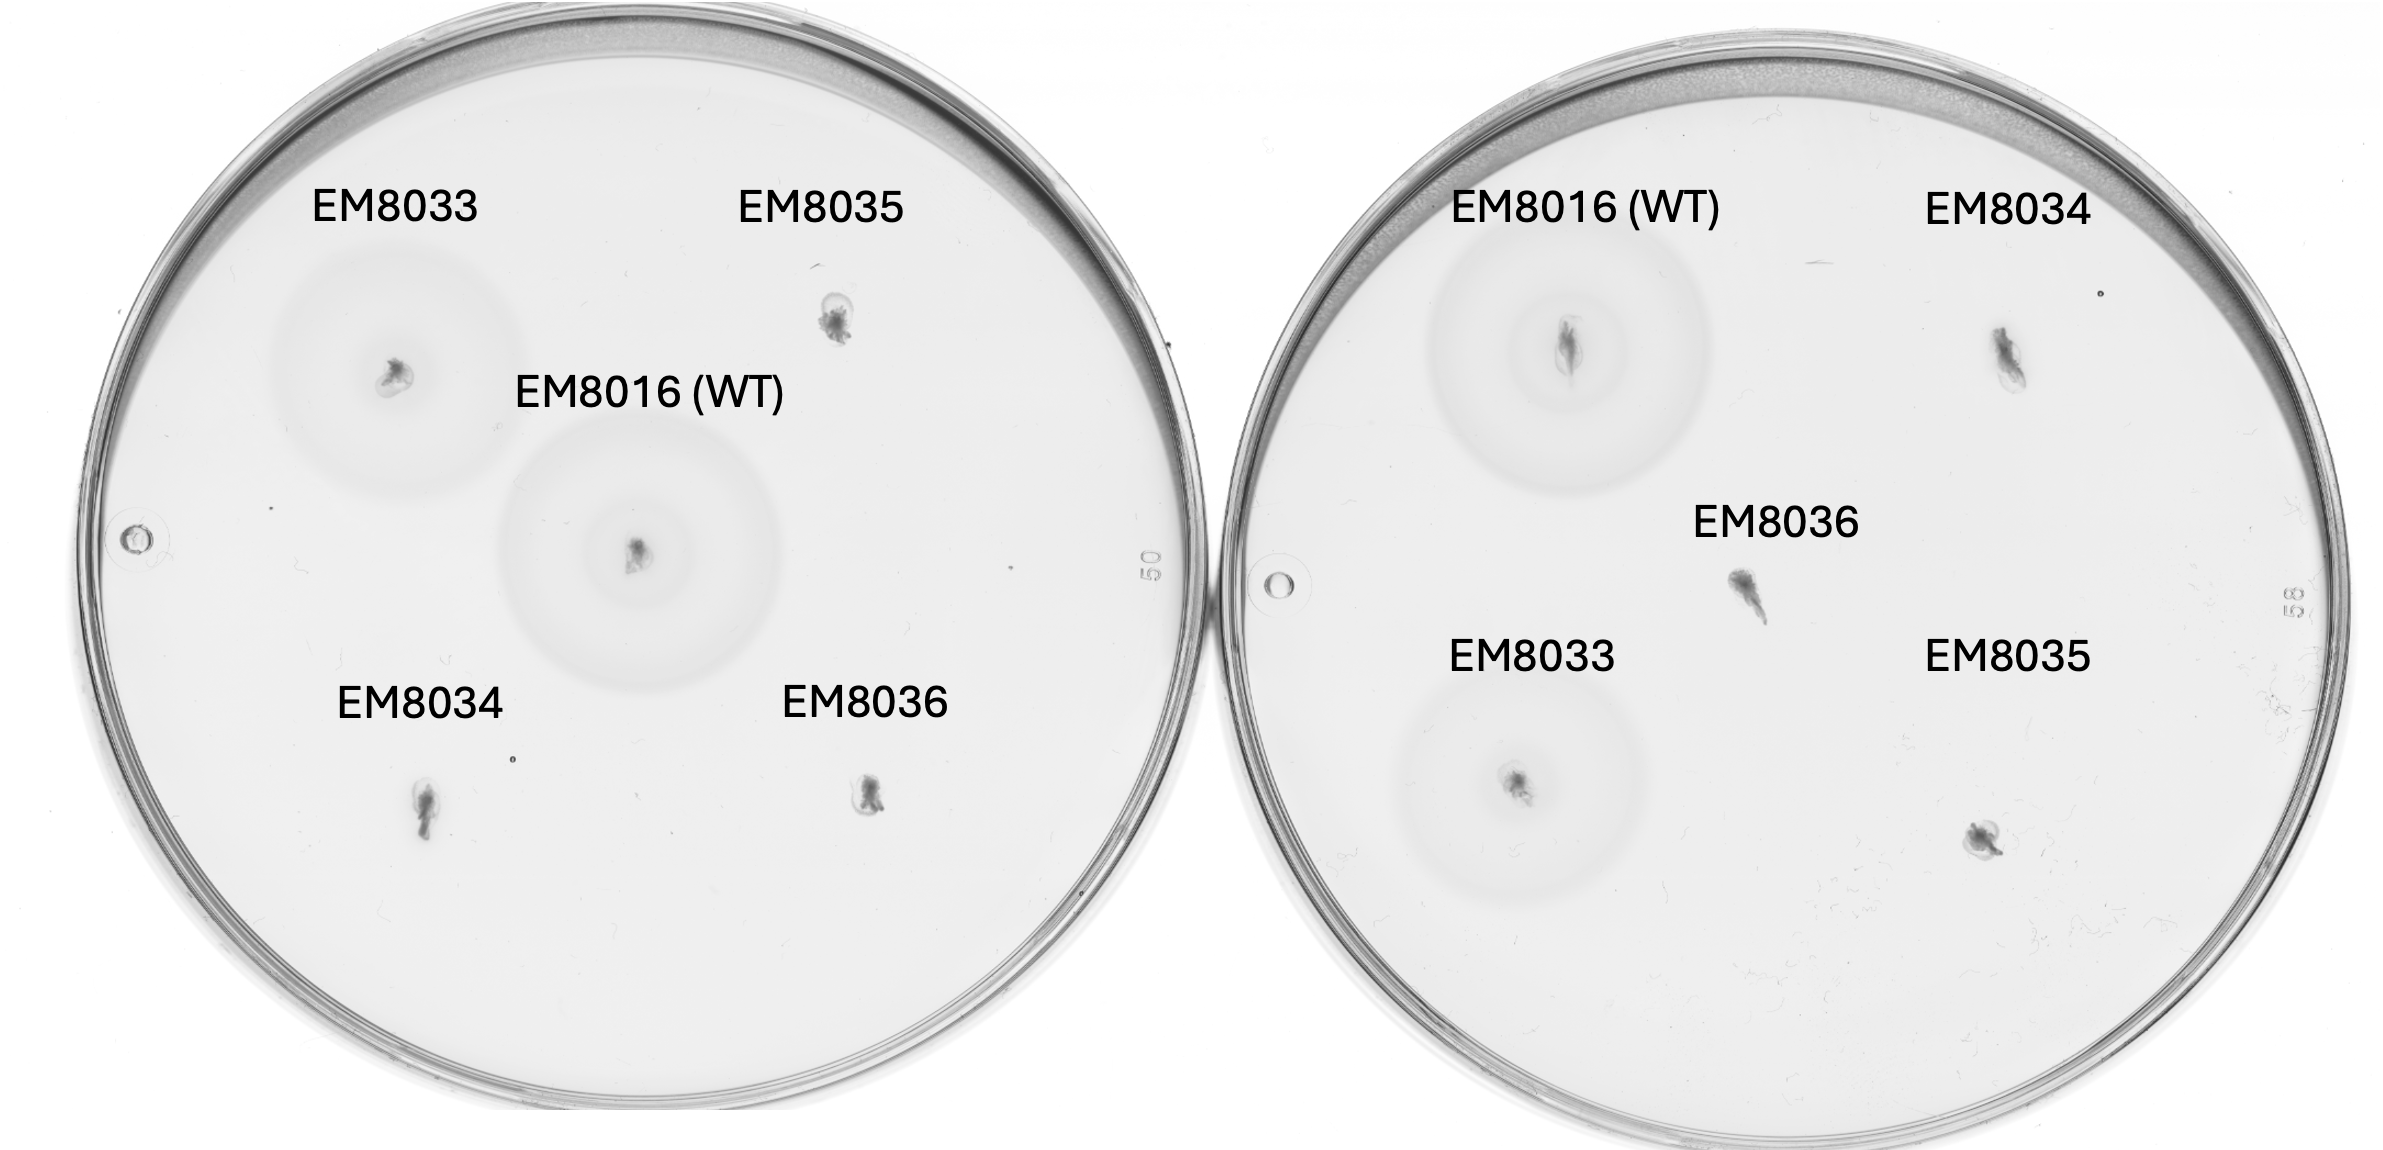
\includegraphics[scale=0.5]{Exp6motility.png}
				\caption{Inokulierte Kulturen in Motility Agar und Inkubation für 4h bei 37°C.}
				\label{fig: Motilitybild}
			\end{figure}
			\begin{figure}[H]
				\centering
				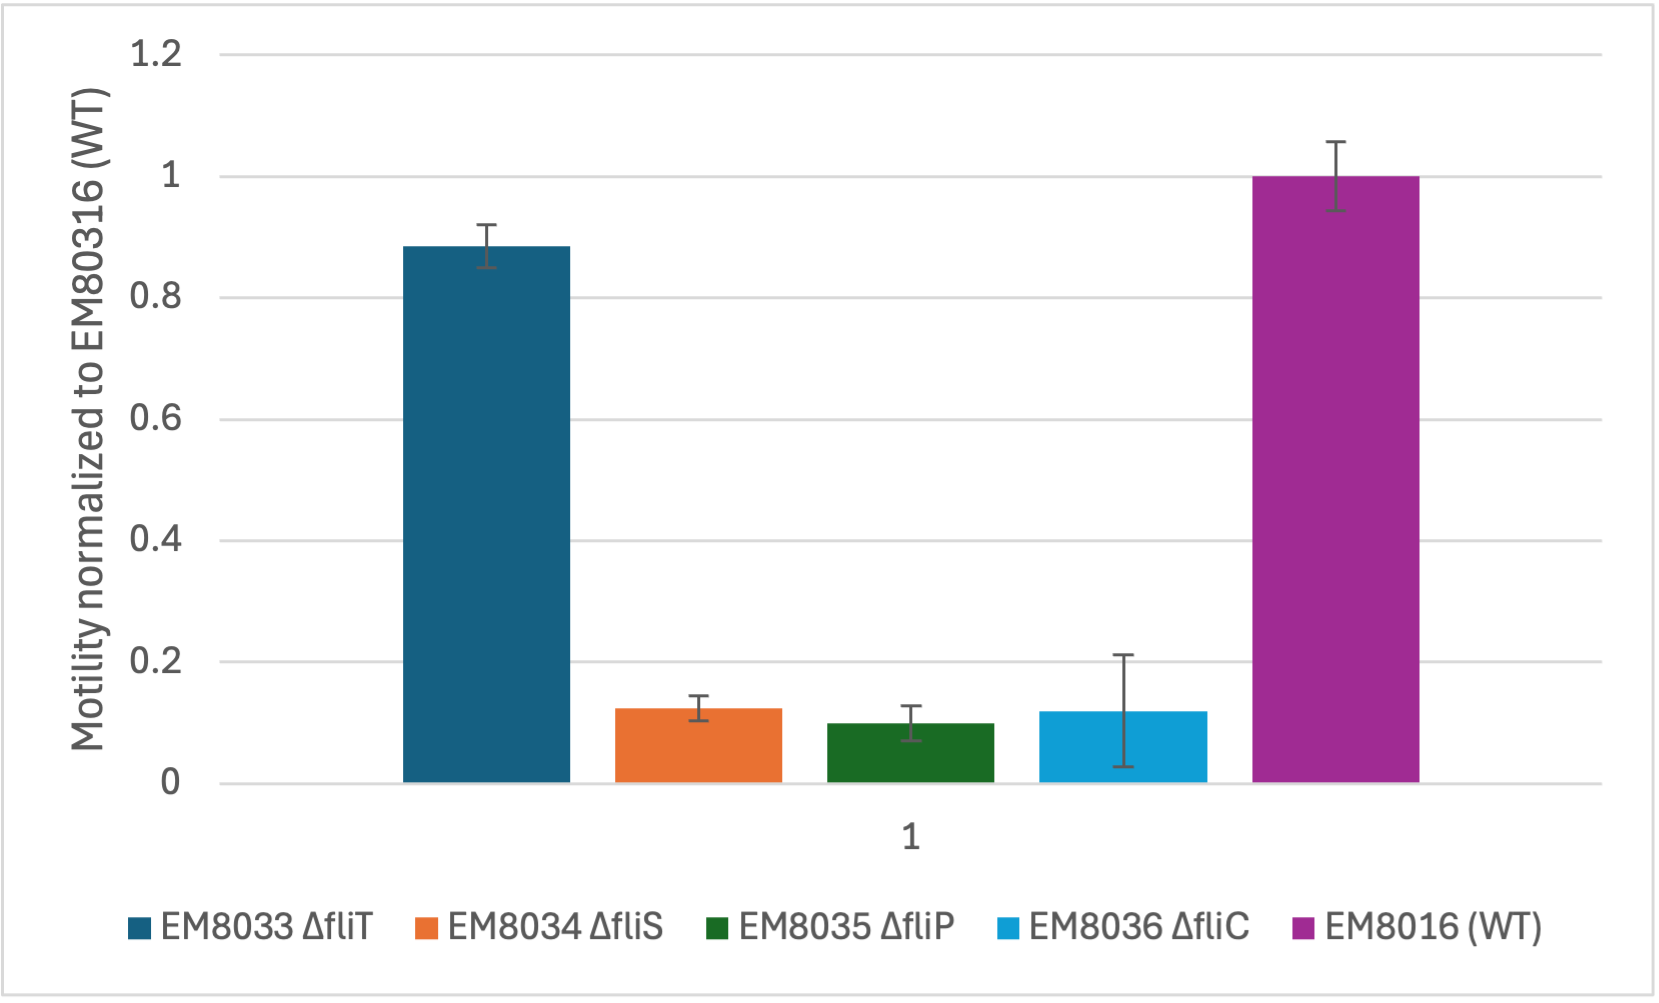
\includegraphics[scale=0.7]{motilitybar.png}
				\caption{Durchschnittliches Durchmesser der Kulturen, die nach 4h bei 37°C sich bewegt haben. Normalisiert wurden die Werte auf dem Wildtyp EM8016 und die Standardabweichung von zwei Platten genommen.}
				\label{fig: Motilitychart}
			\end{figure}
			
			\subsection{Diskussion}
		
		
	\chapter{Dissecting the regulatory mechanism of an unknown flagellar regulator}
		\section{Einleitung}
		
		\section{Methode}
			\begin{table}[H]
			\centering
			\caption{Salmonella-Stämme die für die Untersuchung des unbekannten Flaggella Regulator verwendet wurde.}
			\label{tab: exp8-biologisches Material}
			\begin{tabular}{ccp{5cm}}
				\toprule
				Biologisches Material& Stamm & Phänotyp\\
				\midrule
				\multirow{3}{*}{\parbox[t]{2cm}{Salmonella Wildtyp }}  & \multirow{3}{*}{EM8017} & \multirow{3}{*}{\parbox[t]{5cm}{fliL23026::MudJ-Cm (Km$^R$ in MudJ replaced by FCF = Cm$^R$)}}\\
				&&\\
				&&\\
				\multirow{3}{*}{\parbox[t]{2cm}{Salmonella Mutant}}  & \multirow{3}{*}{EM9900} & \multirow{3}{*}{\parbox[t]{5cm}{fliL23026::MudJ-Cm (Km$^R$ in MudJ replaced by FCF = Cm$^R$) $\Delta$regulator::tetRA}}\\
				&&\\
				&&\\
				&&\\
				\bottomrule			
			\end{tabular}
		\end{table}
		
		\section{Ergebnis}
		
		\section{Diskussion}

	
	
	\chapter{Anhang}
\begin{table}[H]
	\centering
	\caption{Versuch 2: Insertion mutagenesis using the transposable element T-POP. Der Transposon T-POP wurde in die Recipientenzellen des Stammes EM8052 (Table \ref{tab: exp2-biologisches Material}) über Nacht mit einem Phagenlysat TH3468 (Table \ref{tab: exp2-biologisches Material}) transduziert. Anzahl der Kolonien von Gruppe 1-8, die auf MacConkey-lactose Platten mit Tetracyclin und MacConkey-lactose Platten ohne Tetracyclin gewachsen sind, wurden bestimmt und die Anzahl der betroffene Gene ermittelt.}
	\label{tab: exp2-Rohdaten}
	\begin{tabular}{cccccccc}
		\toprule
		\multirow{2}{*}{Gr.} & \multirow{2}{*}{$\#$TcR} & \multirow{2}{*}{Lac$^-$}&\multirow{2}{*}{lac$^-$ (beide Platten)} & \multirow{2}{*}{Tc-dep.-Lac$^-$}& \multirow{2}{*}{Tc-dep.Lac$^+$}& \multirow{2}{*}{Ratio: $\frac{Lac^-}{\#TcR}$}&\multirow{2}{*}{\parbox[*]{1.2cm}{Genes affected}}\\
		&&&&&&&\\
		\midrule
		1 & 246 & 5 & 3 & 2 & 0 & 5/246 & 81\\
		2 & 77 & 1 & 0 & 0 & 1 & 1/77 & 52\\
		3 & 115 & 1 & 1 & 0 & 0 & 1/115& 35\\
		4 & 93 & 2 & 1 & 1 & 0 & 2/93 & 86\\
		5 & 33 & 1 & 1 & 0 & 0 & 1/33& 121\\
		6 & 95 & 0 & 0 & 0 & 0 & NA & NA\\
		7 & 106 & 1 & 1 & 0 & 0 & 1/106 & 38\\
		8 & 274 & 6 & 5 & 1 & 0 & 6/274 & 88\\
		\bottomrule			
	\end{tabular}
\end{table}
	
	
	
	\addcontentsline{toc}{section}{Bibliography}
	\bibliographystyle{plainurl}
	\nocite{*}
	\bibliography{Literatur}
	\newpage
\end{document}